% === T04 - Arquitectura de Procesadores ===
% David Alejandro Gonzalez Marquez
% fokerman@gmail.com
% https://github.com/fokerman/fpgaSoftcoreProgrammingCourse

\RequirePackage[2020-02-02]{latexrelease}

\documentclass[aspectratio=169]{beamer}
\usepackage{../packages}

\newcommand{\na}{\cellcolor{naranjauca}}
\newcommand{\gm}{\cellcolor{gray!50}} 

\title{\Huge Arquitectura de Procesadores}
\author{David Alejandro González Márquez}
\institute{Programación de softcores en FPGAs\\
Programa de Profesoras/es Visitantes\\
Departamento de computación\\
Universidad de Buenos Aires}


\date{}

\begin{document}

\begin{frame}[plain]
    \titlepage
    \begin{textblock}{110}(25,80)
    \begin{tcolorbox}[size=small,width=\textwidth,colback={gray!30},title={}]
    \begin{center}
     \scriptsize Clase disponible en: \url{https://github.com/fokerman/fpgaSoftcoreProgrammingCourse}
    \end{center}
    \end{tcolorbox}
    \end{textblock}
\end{frame}

\begin{frame}[t,fragile]
    \frametitle{Instruction Set Architecture (ISA)}
    \begin{block}{\textbf{Instruction Set Architecture (ISA)}}
    Es la interfaz entre los comandos de \emph{software} y el \emph{hardware} que lo lleva a cabo.
    \end{block}
    \pause
    El ISA especifica:
    \begin{itemize}
    \item<3-> \textbf{La organización de la Memoria}
      \begin{itemize}
       \item Espacio de direcciones ($2^{32}$, $2^{48}$, $2^{64}$, ...).
       \item Unidad direccionable (8 bits, 16 bits, 32 bits, ...).
       \item Orden de los datos (\emph{big-endian} o \emph{little-endian}).
      \end{itemize}
    \item<4-> \textbf{El conjunto de Registros}
    \begin{itemize}
     \item Cantidad e indentificación de registros (R0, R1, R2, ... o EAX, EBX, ECX, ...).
     \item Tipos de uso de registros (dedicados o de propósito general).
    \end{itemize}
    \item<5-> \textbf{El conjunto de Instrucciones}
    \begin{itemize}
     \item Codificación de instrucciones (tamaño fijo o variable, opcodes, predicados, ...).
     \item Tipos de datos (int8, int16, int32, float, double, ...).
     \item Modos de direccionamiento (directo, indirecto, indexado, ...).
     \item Descripción de operaciones (add, sub, or, and, not, ...).
    \end{itemize}
    \end{itemize}
\end{frame}

\begin{frame}[t,fragile]
    \frametitle{Instruction Set Architecture (ISA)}
    \begin{block}{\textbf{Instruction Set Architecture (ISA)}}
    Es la interfaz entre los comandos de \emph{software} y el \emph{hardware} que lo lleva a cabo.
    \end{block}
    El ISA especifica:
    \begin{itemize}
    \item<2-> \textbf{Mecanismos de entrada/salida}
    \begin{itemize}
     \item Espacios de memoria independientes o compartidos (in, out).
     \item Mecanismos de interrupciones.
    \end{itemize}
    \item<3-> \textbf{Soporte de sistemas}
    \begin{itemize}
     \item Administración de memoria.
     \item Administración de procesos.
     \item Administración de energía.
     \item Administración de modos de operación.
     \item Administración de hardware.
    \end{itemize}
    \end{itemize}
\end{frame}

\begin{frame}[t,fragile]
    \frametitle{Modelo de Von Neumann: Componentes básicos}
    \textbf{John von Neumann} propuso el modelo fundamental de una computadora para el procesamiento de programas en 1946.\\
    \bigskip
    \pause
    \textcolor{verdeuca}{Este modelo está basado en dos \textbf{principios}:}
    \begin{itemize}
    \item<2-> \textbf{Programa almacenado}\\
    \begin{itemize}
     \item Las instrucciones se guardan en una \textcolor{verdeuca}{\textbf{arreglo lineal de memoria}}.
     \item La \textcolor{verdeuca}{\textbf{memoria es unificada}} entre datos e instrucciones. 
     \item La \textcolor{verdeuca}{\textbf{interpretación}} de los datos almacenados depende de señales de control.
    \end{itemize}
    \item<3-> \textbf{Programa secuencial}\\
    \begin{itemize}
     \item Una instrucción es procesada \textcolor{verdeuca}{\textbf{por unidad de tiempo}} (fetch, decode, execute).
     \item El PC define la \textcolor{verdeuca}{\textbf{próxima instrucción}} a ejecutar.
     \item El PC aumenta \textcolor{verdeuca}{\textbf{secuencialmente}} (excepto para las instrucciones de control).
    \end{itemize}
    \end{itemize}
    \bigskip
    \uncover<4->{
    \textcolor{verdeuca}{y está compuesto de 5 \textbf{componentes básicos}:}
    \begin{center}
    \begin{tabular}{ll}
    \begin{minipage}{6cm}
        \begin{itemize}
        \setlength\itemsep{0cm}
        \item Memoria
        \item Procesador
        \item Unidad de control
        \end{itemize}
    \end{minipage}
    &
    \begin{minipage}{6cm}
        \begin{itemize}
        \setlength\itemsep{0cm}
        \item Interfaz de entrada
        \item Interfaz de salida
        \end{itemize}
    \end{minipage}
    \\
    \end{tabular}
    \end{center}
    }
\end{frame}

\begin{frame}[t,fragile]
    \frametitle{Arquitecturas de procesadores}
    \begin{textblock}{140}(14,12)
    \small
    \begin{itemize}
    \setlength\itemsep{0cm}
    \item[1974]<1-> \textbf{8080} - 8 bits - Intel
    \item[1974]<1-> \textbf{6800} - 8 bits - Motorola
    \item[1974]<1-> \textbf{Z80} - 8 bits - Zilog
    \item[1975]<1-> \textbf{MOS 6502} - 8 bits - MOS Technology.
    \item[1978]<2-> \textbf{x86, x86-64, AMD64} - 16, 32, 64 bits - Intel/AMD.
    \item[1979]<2-> \textbf{68000} - 16, 32 bits - Motorola
    \item[1983]<3-> \textbf{ARM (Advanced RISC Machine)} - 32, 64 bits - Licenciado por ARM Holdings.
    \item[1984]<3-> \textbf{MIPS} - 32, 64 bits - MIPS Technologies (comprado por Hewlett Packard)
    \item[1986]<3-> \textbf{PA-RISC} - 32 bits - Hewlett Packard
    \item[1987]<3-> \textbf{SPARC} - 32 bits - Sun Microsystems (comprado por Oracle)
    \item[1992]<4-> \textbf{DEC Alpha} - 64 bits - Digital (comprado por Hewlett Packard)
    \item[1992]<4-> \textbf{PowerPC} - 32, 64 bits - IBM
    \item[2001]<4-> \textbf{Itanium} - 64 bits - Hewlett Packard y Intel
    \item[2007]<4-> \textbf{Cell} - 32, 64 bits - IBM
    \end{itemize}
    \end{textblock}
\end{frame}

\begin{frame}[t,fragile]
    \frametitle{LC-3: Ejemplo de una máquina von Neumann}
    \begin{textblock}{70}(10,10)
    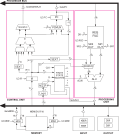
\includegraphics[scale=0.55]{imgBook/lc3_datapath_simple_C4F3_PyP.pdf}
    \end{textblock}
    \begin{textblock}{60}(85,14)
    \small
    La LC-3 es una computadora simple que presentaremos para estudiar su funcionamiento.\\
    \bigskip
    \uncover<2->{
    \textcolor{verdeuca}{En el datapath se pueden identificar todos los componentes básicos de una máquina von Neumann.}\\
    }
    \bigskip
    \uncover<3->{
    Notar que:\\
    \begin{itemize}
    \item Las flechas de punta negra identifican el \textbf{camino de los datos}.\\
    \item Las flechas de punta blanca identifican las \textbf{señales de control}.\\
    \end{itemize}
    }
    \end{textblock}
\end{frame}

\begin{frame}[t,fragile]
    \frametitle{LC-3: Ejemplo de una máquina von Neumann}
    \begin{textblock}{70}(10,10)
    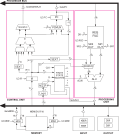
\includegraphics[scale=0.55]{imgBook/lc3_datapath_simple_C4F3_PyP.pdf}
    \end{textblock}
    \begin{textblock}{65}(85,12)
    \textbf{MEMORY}\\
    \small
    Consiste en un arreglo de posiciones de memoria accesible por dos registros.
    \bigskip
    \begin{enumerate}
    \item<2-> \textbf{Memory Address Register (\texttt{MAR})}\\ Contiene la dirección de memoria que se busca acceder.
    \item<3-> \textbf{Memory Data Register (\texttt{MDR})}\\ Contiene el contenido de la posición de memoria, tanto para lectura como escritura.
    \end{enumerate}
    \bigskip
    \uncover<4->{
    \textcolor{gray}{Espacio direccionable dado por \texttt{MAR} de 16 bits, es decir $2^{16}$ posiciones de memoria.}\\
    \textcolor{gray}{Unidad direccionable dado por \texttt{MDR} de 16 bits.}
    }
    \end{textblock}
\end{frame}

\begin{frame}[t,fragile]
    \frametitle{LC-3: Ejemplo de una máquina von Neumann}
    \begin{textblock}{70}(10,10)
    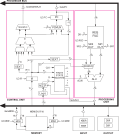
\includegraphics[scale=0.55]{imgBook/lc3_datapath_simple_C4F3_PyP.pdf}
    \end{textblock}
    \begin{textblock}{60}(85,12)
    \textbf{INPUT/OUTPUT}\\
    \small
    Consiste en un teclado y un monitor.\\
    \uncover<2->{
    \textcolor{verdeuca}{\textbf{Keyboard}}
    \begin{itemize}
    \setlength\itemsep{0cm}
     \item \footnotesize \textbf{Keyboard data register (KBDR)}\\ Mantiene el código ASCII de la tecla presionada.
     \item \footnotesize \textbf{Keyboard status register (KBSR)}\\ Mantiene información del estado de la tecla presionada.
    \end{itemize}
    }
    \uncover<3->{
    \textcolor{verdeuca}{\textbf{Monitor}}
    \begin{itemize}
    \setlength\itemsep{0cm}
    \item \footnotesize \textbf{Display data register (DDR)}\\ Mantiene el código ASCII del caracter enviado a pantalla.
     \item \footnotesize \textbf{Display status register (DSR)}\\ Mantiene información del estado del caracter enviado.
    \end{itemize}
    }
    \end{textblock}
\end{frame}

\begin{frame}[t,fragile]
    \frametitle{LC-3: Ejemplo de una máquina von Neumann}
    \begin{textblock}{70}(10,10)
    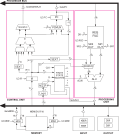
\includegraphics[scale=0.55]{imgBook/lc3_datapath_simple_C4F3_PyP.pdf}
    \end{textblock}
    \begin{textblock}{60}(85,12)
    \textbf{THE PROCESSING UNIT}\\
    \small
    \bigskip
    Consiste de dos partes:
    \begin{itemize}
     \item<2-> \textbf{ALU} encargada de realizar las operaciones aritméticas y lógicas.\\
    \textcolor{gray}{En la LC-3, la ALU está limitada para realizar solo la operación aritmética suma y las operaciones lógicas AND y NOT.}
     \item<3-> \textbf{Banco de registros} encargado de almacenar datos temporariamente.\\
    \textcolor{gray}{Contiene 8 registros de propósi to general, un puerto de escritura y dos puertos de lectura.}\\
    \end{itemize}
    \end{textblock}
\end{frame}

\begin{frame}[t,fragile]
    \frametitle{LC-3: Ejemplo de una máquina von Neumann}
    \begin{textblock}{70}(10,10)
    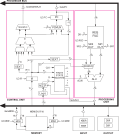
\includegraphics[scale=0.55]{imgBook/lc3_datapath_simple_C4F3_PyP.pdf}
    \end{textblock}
    \begin{textblock}{60}(85,12)
    \textbf{THE CONTROL UNIT}\\
    \small
    \bigskip
    Contiene en todas las estructuras y módulos necesarios para \textbf{administrar el procesamiento }de la computadora.\\
    \bigskip
    \uncover<2->{
    La parte más importante es la \textbf{máquina de estados} que controla el funcionamiento de todo el sistema.\\
    \vspace{0.2cm}
    \textcolor{verdeuca}{Se ocupa de llevar paso a paso \textbf{el ciclo de instrucción} para todas las instrucciones soportadas por el procesador.}\\
    }
    \bigskip
    \uncover<3->{
    \textcolor{gray}{Notar que todas las entradas en la máquina de estados son datos, además del reloj, y las salidas son señales de control.}\\
    }
    \end{textblock}
\end{frame}

\begin{frame}[t,fragile]
    \frametitle{Procesamiento de Instrucciones}
    \textcolor{verdeuca}{La unidad más básica de procesamiento es la \textbf{instrucción}.}\\
    \uncover<2->{
    Está compuesta principalmente de dos partes:
    \begin{itemize}
    \setlength\itemsep{0cm}
     \item \textbf{opcode}: Indica la instrucción a realizar.
     \item \textbf{operands}: Indica sobre que valores se va a ejecutar.
    \end{itemize}
    }
    \uncover<3->{
    En general existen cuatro tipos de instrucciones:
    \begin{itemize}
    \setlength\itemsep{0cm}
    \item \textcolor{verdeuca}{Instrucciones de \textbf{operación} o calculo.}
    \item \textcolor{verdeuca}{Instrucciones de \textbf{movimiento} de datos.}
    \item \textcolor{verdeuca}{Instrucciones de cambio en el \textbf{control} de flujo.}
    \item \textcolor{verdeuca}{Instrucciones \textbf{especiales}.}
    \end{itemize}
    }
    \bigskip
    \uncover<4->{
    \textcolor{naranjauca}{En la LC-3 las instrucciones son de \textbf{tamaño fijo de 16 bits}.}\\
    \begin{itemize}
    \item \textcolor{naranjauca}{\textbf{Bits \texttt{[15:12]}}}: Contienen el opcode.
    \item \textcolor{naranjauca}{\textbf{Bits \texttt{[11:0]}}}: Se utilizan para identificar los operandos.
    \end{itemize}
    }
    \begin{textblock}{53}(100,7)
    \uncover<4->{
    \begin{block}{\footnotesize Ejemplo instrucción \texttt{ADD}}
    \scriptsize
    Dos tipos posibles de codificación:
    \begin{center}
    \texttt{R6 $\leftarrow$ R2 + R6}\\ \vspace{0.1cm}
    \includegraphics[scale=0.45]{imgBook/lc3_add_instruction_example_PyP-layer1.pdf}
    \end{center}
    \begin{center}
    \texttt{R6 $\leftarrow$ R2 + 6}\\ \vspace{0.1cm}
    \includegraphics[scale=0.45]{imgBook/lc3_add_instruction_example_PyP-layer2.pdf}
    \end{center}
    \textcolor{naranjauca}{\textbf{Bits \texttt{[15:12]}}}: \texttt{0001}, corresponde al ADD.\\
    \textcolor{naranjauca}{\textbf{Bits \texttt{[11:9]}}}: Registro destino.\\
    \textcolor{naranjauca}{\textbf{Bits \texttt{[8:6]}}}: Registro operando 1.\\
    \textcolor{naranjauca}{\textbf{Bits \texttt{[5]}}}: Indica tipo de operando 2.\\
    \textcolor{naranjauca}{\textbf{Bits \texttt{[2:0]}}}: Registro operando 2, si \texttt{Bits[5]=0}.\\
    \textcolor{naranjauca}{\textbf{Bits \texttt{[4:0]}}}: Inmediato con signo extendido como operando 2, si \texttt{Bits[5]=1}.\\
    \end{block}
    }
    \end{textblock}
\end{frame}

\begin{frame}[t,fragile]
    \frametitle{Ciclo de Instrucción}
    Las instrucciones son procesadas de forma secuencial una después de la otra.\\
    \uncover<2->{
    \textcolor{verdeuca}{Si bien internamente podemos romper esté contrato,\\
    a nivel de la arquitectura del sistema lo debemos respetar.}\\
    }
    \bigskip
    \uncover<3->{
    De forma general el ciclo de instrucción consiste en las siguientes etapas:
    \begin{enumerate}
    \item \textcolor{naranjauca}{FETCH}
    \item \textcolor{naranjauca}{DECODE}
    \item \textcolor{naranjauca}{EVALUATE ADDRESS}
    \item \textcolor{naranjauca}{FETCH OPERANDS}
    \item \textcolor{naranjauca}{EXECUTE}
    \item \textcolor{naranjauca}{STORE RESULT}
    \end{enumerate}
    }
    \uncover<4->{
    \small
    \begin{center}
    \textcolor{gray}{Cada etapa puede requerir más de un ciclo de reloj\\ o incluso puede no ser necesaria para resolver la instrucción.}
    \end{center}
    }
\end{frame}

\begin{frame}[t,fragile]
    \frametitle{Ciclo de Instrucción: FETCH}
    \small
    \begin{block}{\vspace*{-3ex}}
    \textbf{FETCH}: Obtiene la instrucción de memoria y la carga en el registro IR.
    \end{block}
    \bigskip
    \uncover<2->{
    Pasos:
    \begin{enumerate}
     \item Carga el registro \texttt{MAR} con el contenido de \texttt{PC} y simultáneamente incrementa el \texttt{PC}.
     \item Lee la memoria y guarda el contenido en el registro \texttt{MDR}.
     \item Carga en el registro \texttt{IR} el contenido de \texttt{MDR}.
    \end{enumerate}
    }
    \bigskip
    \uncover<3->{
    \textcolor{gray}{Notar que el \texttt{PC} siempre queda apuntando a la \textbf{próxima instrucción} que debe ser ejecutada.}\\
    }
    \bigskip
    \uncover<4->{
    \textcolor{gray}{Dependiendo de la unidad direccionable de la memoria y el tamaño de la instrucción puede ser necesario \textbf{leer más de un valor de memoria}.
    Incluso puede ser necesario decodificar parcialmente la instrucción para decidir si se debe leer o no los próximos datos de memoria.}
    }
\end{frame}

\begin{frame}[t,fragile]
    \frametitle{Ciclo de Instrucción: DECODE}
    \small
    \begin{block}{\vspace*{-3ex}}
    \textbf{DECODE}: Evaluá la instrucción para determinar que acción realizar a nivel de microarquitectura.
    \end{block}
    \bigskip
    \uncover<2->{
    En LC-3 un decodificador de 4 entradas identifica los \textbf{16 opcodes posibles} (\texttt{IR [15:12]}).\\
    \textcolor{verdeuca}{Dependiendo el opcode identificado, se interpretan los 12 bits restantes.}\\
    }
    \bigskip
    \uncover<3->{
    La decodificación puede incluir \textbf{generar señales de control o de datos} que dependiendo de la instrucción pueden ser utilizados o no.\\
    }
    \bigskip
    \uncover<4->{
    \textcolor{gray}{Un ejemplo para nuestra máquina puede ser el bit 5 de \texttt{IR} que solo se utiliza sí la instrucción debe utilizar un segundo parámetro.}
    }
\end{frame}

\begin{frame}[t,fragile]
    \frametitle{Ciclo de Instrucción: EVALUATE ADDRESS}
    \small
    \begin{block}{\vspace*{-3ex}}
    \textbf{EVALUATE ADDRESS}: Calcula la dirección de memoria necesaria para procesar la instrucción.
    \end{block}
    \uncover<2->{
    En LC-3, para las instrucciones que requieren acceder a memoria, en esta etapa se calcula la dirección de memoria relativa al \texttt{PC} actual.\\
    }
    \bigskip
    \uncover<3->{
    \textit{Por ejemplo:}\\
    La instrucción \texttt{LD}, lee un valor de memoria y almacena su contenido en un registro.\\
    \textcolor{verdeuca}{La etapa de EVALUATE ADDRESS, toma de la instrucción un valor inmediato de 9 bits
    que se utiliza como un \textbf{desplazamiento} sobre el valor actual del \texttt{PC},
    calculando el valor absoluto de la dirección de memoria.}\\
    }
    \bigskip
    \uncover<4->{
    \textcolor{gray}{Utilizar un registro como base de los desplazamientos en memoria es una prática común en las arquitecturas de procesadores,
    ya que permite reducir la cantidad de bits necesarios para codificar el valor absoluto de una dirección de memoria dentro de una instrucción.}\\
    }
\end{frame}

\begin{frame}[t,fragile]
    \frametitle{Ciclo de Instrucción: FETCH OPERANDS}
    \small
    \begin{block}{\vspace*{-3ex}}
    \textbf{FETCH OPERANDS}: Trae de memoria los datos requeridos para procesar la instrucción.
    \end{block}
    \uncover<2->{
    En está etapa se leen los operandos de memoria.\\
    \textcolor{verdeuca}{En arquitecturas con modos de direccionamiento más complejos, es la encargada de leer los datos.\\
    Por ejemplo, en indirecto a registro, lee los datos para luego usarlos como operandos.}\\
    }
    \bigskip
    \uncover<3->{
    En LC-3, para la instrucción \texttt{LD} está etapa carga el registro \texttt{MAR} con la dirección absoluta y luego carga el contenido de \texttt{MDR} en el registro destino.\\
    \vspace{0.2cm}
    Para la instrucción \texttt{ADD} en cambio, se ocupa de obtener los registros del banco de registros.\\
    }
    \bigskip
    \uncover<4->{
    \textcolor{gray}{En microarquitecturas más complejas, la etapa de obtener los operandos se realizar fuera de orden.\\
    Luego, a medida que se calculan los operandos, las instrucciones son ejecutadas.}
    }
\end{frame}

\begin{frame}[t,fragile]
    \frametitle{Ciclo de Instrucción: EXECUTE}
    \small
    \begin{block}{\vspace*{-3ex}}
    \textbf{EXECUTE}: Consiste en la ejecución de la operación codificada por la instrucción.
    \end{block}
    \uncover<2->{
    En LC-3, para la instrucción \texttt{ADD} correspondería a la etapa en que los operandos son cargados en la ALU y el resultado de la operación es generado.\\
    }
    \bigskip
    \uncover<3->{
    \textcolor{gray}{Dependiendo de la instrucción, está etapa \textbf{puede no ser necesaría}, ya que no todas las operaciones requieren la ALU o acceder a registros para hacer su operación.}\\
    }
    \bigskip
    \uncover<4->{
    \textcolor{verdeuca}{Incluso, dependiendo del \emph{datapath}, es posible que está etapa sea necesaria pero sin hace nada útil.}
    }
    
\end{frame}

\begin{frame}[t,fragile]
    \frametitle{Ciclo de Instrucción: STORE RESULT}
    \small
    \begin{block}{\vspace*{-3ex}}
    \textbf{STORE RESULT}: Almacena los resultados de la operación en el lugar que fueron designados.
    \end{block}
    \uncover<2->{
    Esta última etapa suele no ser necesaria en microarquitecturas muy simples.\\
    }
    \bigskip
    \uncover<3->{
    En LC-3 como en otras computadoras, la instrucción ADD puede cargar los operandos, realizar la operación y guardar el resultado en un solo ciclo.\\
    }
    \bigskip
    \uncover<4->{
    \textcolor{gray}{Es importante reconocer está etapa en un ciclo de instrucción general, ya que se puede no disponer del recurso donde escribir el resultado de la operación.\\}
    }
\end{frame}

\begin{frame}[t,fragile]
    \frametitle{Cambios en la ejecución secuencial de instrucciones}
    \small
    \textcolor{verdeuca}{Hasta ahora nuestra máquina ejecuta instrucciones de forma \textbf{secuencial}, una detrás de la otra.}\\
    \vspace{0.2cm}
    El cálculo de la dirección de la nueva instrucción se realiza en la etapa de \texttt{Fetch}.\\
    \bigskip
    \uncover<2->{
    Las instrucciones de control se ocupan de \textbf{pisar el valor del \texttt{PC}} con un nuevo dato obtenido\\
    en la etapa de \texttt{Execute}.\\
    }
    \bigskip
    \uncover<3->{
    Existen tres tipos de instrucciones de control:
    }
    \begin{itemize}
     \item<3-> \textcolor{naranjauca}{\textbf{Salto incondicional}}: Cambia el PC remplazandolo por un valor calculado o estático.\\
     \textcolor{gray}{En LC-3, la instrucción: \texttt{JMP} (\emph{jump})}
     \item<4-> \textcolor{naranjauca}{\textbf{Salto condicional}}: Cambia el PC si se cumple una determinada condición.\\
     \textcolor{gray}{En LC-3, la instrucción: \texttt{BR} (\emph{conditional branch})}
     \item<5-> \textcolor{naranjauca}{\textbf{Llamado o retorno de subrutina}}: Cambia el PC y resguarda el PC remplazado.\\ Luego puede retornar el control al PC que fue resguardado.\\
     \textcolor{gray}{En LC-3, las instrucciones: \texttt{JSR(R)}, (\emph{JumpSubRutine}), \texttt{RET} (\emph{return})}
    \end{itemize}
\end{frame}

\begin{frame}[t,fragile]
    \frametitle{Control del ciclo de instrucción}
    \begin{textblock}{72}(12,12)
    \small
    Es controlado por una \textbf{máquina de estados}.\\
    \textcolor{verdeuca}{Cada estado representa un conjunto de señales que se envían a los diferentes componentes del \emph{datapath}.}\\
    \vspace{0.2cm}
    \uncover<2->{
    \textcolor{gray}{Las flechas entre los diferentes estados representan las \textbf{transiciones} de un estado a otro. Estas pueden ser secuenciales o depender de alguna condición.}\\
    }
    \vspace{0.2cm}
    \uncover<3->{
    \textbf{La etapa de \texttt{Fetch}} corresponden a los primeros tres estados.\\
    }
    \vspace{0.2cm}
    \uncover<4->{
    \textbf{La etapa de \texttt{Decode}} demora un ciclo representado por el estado 4, saltando al estado correspondiente dependiendo de la instrucción decodificada.
    }
    \vspace{-0.2cm}
    \uncover<5->{
    \begin{block}{\vspace*{-3ex}}
    \scriptsize
    Esta máquina de estados puede ser implementada de diferentes formas. Sin embargo, la forma más simple, es codificar los estados en una memoria y accederlos secuencialmente.
    Adicionando lógica para saltar a estados según datos de control como el opcode.
    \end{block}
    }
    \end{textblock}
    \begin{textblock}{65}(95,12)
    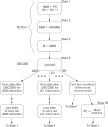
\includegraphics[scale=0.55]{imgBook/lc3_state_machine_C4F4_PyP.pdf}
    \end{textblock}
\end{frame}

\begin{frame}[t,fragile]
    \frametitle{Control del ciclo de instrucción: \small Máquina de estados completa (Sin interrupciones)}
    \begin{center}
    \vspace{-0.4cm}
    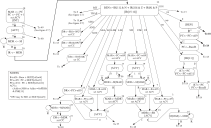
\includegraphics[scale=0.6]{imgBook/lc3_complete_state_machine_ApCF2_PyP_modified.pdf}
    \end{center}
\end{frame}

\begin{frame}[t,fragile]
    \frametitle{Interrupciones (Instrucción \texttt{TRAP})}
    \bigskip
    Los procesadores poseen mecanismos para \textbf{detener el procesamiento} y tomar el control.\\
    \bigskip
    \uncover<2->{
    \textcolor{verdeuca}{El soporte se puede prestar mediante una instrucción o independiente de las instrucciones.\\
    Puede contar con soporte para un vector de interrupciones o una única interrupción.}\\
    }
    \bigskip
    \uncover<3->{
    En LC-3, se cuenta con la instrucción \texttt{TRAP} (\texttt{opcode}=\texttt{1111}) que realiza está tarea.\\
    \begin{center}
    
\includegraphics[scale=0.9]{imgBook/lc3_trap_instruction_PyP.pdf}
    \end{center}
    \textcolor{gray}{
    Los bits [7:0] (\texttt{trapvector}), codifican el vector de interrupciones.\\
    Este valor se usa como índice en la \textbf{tabla de vectores de interrupción} para identificar la rutina.}
    }
\end{frame}

\begin{frame}[t,fragile]
    \frametitle{Conjunto de Instrucciones (\emph{Instruction Set})}
    \begin{textblock}{65}(110,2)
    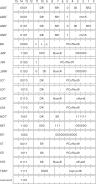
\includegraphics[scale=0.46]{imgBook/lc3_instruction_format_C5F3_PyP.pdf}
    \end{textblock}
    \begin{textblock}{90}(10,12)
    \small
    Los opcode permiten identificar las diferentes instrucciones.\\
    Pueden estar determinados por un conjunto de bits fijo o variable.\\
    \bigskip
    \uncover<2->{
    \textcolor{gray}{
    Se busca que la codificación de instrucciones sea \textbf{regular}.\\
    Los opcode y parámetros siempre en los mismos lugares e interpretados de la misma forma.\\
    Esto simplifica la máquinaria de decodificación.}\\
    }
    \bigskip
    \uncover<3->{
    Puede ser que en algunos casos sea necesario pasar por varias \textbf{etapas de decodificación} para identificar las instrucciones.\\
    }
    \bigskip
    \uncover<4->{
    En LC-3, su ISA cuenta con 15 instrucciones.\\ Cada una identificada por un \textbf{opcode único}.\\
    }
    \bigskip
    \uncover<4->{
    \textcolor{verdeuca}{Se identifican \textbf{diferentes tipos} de instrucciones, que dependen de como los parámetros fueron ordenados.}
    }
    \end{textblock}
\end{frame}

\begin{frame}[t,fragile]
    \frametitle{Tipos de datos}
    \begin{textblock}{65}(100,2)
    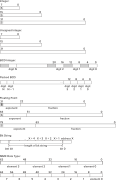
\includegraphics[scale=0.46]{imgBook/data_types_B1_PyP.pdf}
    \end{textblock}
    \begin{textblock}{30}(124,3)
    \scriptsize Tipos de datos soportados por la arquitectura \texttt{x86}
    \end{textblock}
    \begin{textblock}{85}(10,12)
    \small
    Las diferentes instrucciones pueden soportar parámetros en distintos o en un único tipo de datos.\\
    \bigskip
    \uncover<2->{
    \textcolor{verdeuca}{Internamente los distintos tipos de datos se resuelven con máquinaria diferente del procesador, lo que implica diferencias en la performance de las operaciones.}\\
    }
    \bigskip
    \uncover<3->{
    \textcolor{gray}{Los tipos de datos pueden ser tanto iterpretaciones de los bits de registros, como de memoria o incluso registros internos no accesibles por el programador.\\}
    }
    \bigskip
    \uncover<4->{
    En LC-3, solo se soportan datos enteros de tamaño fijo de 16 bits.
    }
    \end{textblock}
\end{frame}

\begin{frame}[t,fragile]
    \frametitle{Modos de direccionamiento}
    Es el mecanismo por el cual se especifica donde se encuentra un operando.\\
    \uncover<2->{
    \textcolor{verdeuca}{Generalmente los operandos pueden estar en tres lugares:}
    \begin{itemize}
    \item En un registro.
    \item En una posición de memoria.
    \item En la instrucción como un literal.
    \end{itemize}
    }
    \bigskip
    \uncover<3->{
    \textcolor{verdeuca}{En LC-3 se soportan 5 modos de direccionamiento:}
    \begin{itemize}
    \item Inmediato o Literal
    \item Registro
    \item Relativo-PC
    \item Indirecto
    \item Base-Desplazamiento
    \end{itemize}
    }
\end{frame}

\begin{frame}[t,fragile]
    \frametitle{Instrucciones de operación}
    \begin{textblock}{65}(85,5) \includegraphics[scale=0.6]{imgBook/lc3_datapath_simple_C4F3_PyP_Operaciones-layer2.pdf} \end{textblock}
    \begin{textblock}{65}(85,5) \includegraphics[scale=0.6]{imgBook/lc3_datapath_simple_C4F3_PyP_Operaciones-layer1.pdf} \end{textblock}
    \begin{textblock}{70}(10,12)
    \small
    Las operaciones aritméticas como ADD, SUB, NEG, MUL, DIV, o lógicas como AND, OR, NOT, XOR son ejemplos básicos de instrucciones.\\
    \uncover<2->{
    \textcolor{gray}{Pueden operar con un solo operando como NEG o NOT, o con dos o más parámetros.}\\
    }
    \bigskip
    \uncover<3->{
    \textcolor{verdeuca}{Resolver los parámetros se reliza a traves de diferentes modos de direccionamiento.}\\
    \begin{itemize}
     \item \textcolor{verdeuca}{\textbf{Inmediatos}: Decodificarlos de la instrucciones o usar constantes.}
     \item \textcolor{verdeuca}{\textbf{Registros}: Se debe poder identificarlos.}
     \item \textcolor{verdeuca}{\textbf{Memoria}: Generar u obtener la dirección, acceder al dato para escritura o lectura.}
    \end{itemize}
    }
    \uncover<4->{
    En LC-3, solo se cuenta con tres instrucciones de este tipo: ADD, AND, y NOT.\\
    }
    \end{textblock}
\end{frame}

\begin{frame}[t,fragile]
    \frametitle{Instrucciones de operación}
    \begin{textblock}{65}(90,5) \includegraphics[scale=0.6]{imgBook/lc3_instructions_code-layer1.pdf} \end{textblock}
    \begin{textblock}{65}(90,18) \includegraphics[scale=0.6]{imgBook/lc3_instructions_datapath-layer1.pdf} \end{textblock}
    \begin{textblock}{75}(10,12)
    \small
    La instrucción NOT (\texttt{opcode} = \texttt{1001}) opera con dos parámetros, un registro fuente y otro destino.\\
    \bigskip
    \uncover<2->{
    Utilizamos los bits [8:6] para especificar el registro fuente y los bits [11:9] para el registro destino.\\
    }
    \bigskip
    \uncover<2->{
    Por convención los bits [5:0] deben contener todos un 1.\\
    }
    \bigskip
    \uncover<3->{
    \textcolor{gray}{
    En el ejemplo se realiza un NOT de \texttt{R5} y se almacena el resultado en el registro \texttt{R3}.
    Además los flags son alterado según el resultado de la operación.\\}
    \bigskip
    \textcolor{verdeuca}{Notar que ambos parárametros pueden ser el mismo registro.}
    }
    \end{textblock}
\end{frame}

\begin{frame}[t,fragile]
    \frametitle{Instrucciones de operación}
    \begin{textblock}{65}(90,5) \includegraphics[scale=0.6]{imgBook/lc3_instructions_code-layer2.pdf} \end{textblock}
    \begin{textblock}{65}(86,18) \includegraphics[scale=0.6]{imgBook/lc3_instructions_datapath-layer2.pdf} \end{textblock}
    \begin{textblock}{70}(10,12)
    \small
    En LC-3, las instrucciones ADD (opcode = 0001) y AND (opcode = 0101) 
    realizan operaciones binarias, que requieren como entrada dos datos de 16 bits.\\
    \bigskip
    \uncover<2->{
    \textcolor{verdeuca}{Tiene dos sabores, donde uno de sus parámetros puede ser es un valor inmediato o un registro.}\\
    }
    \bigskip
    \uncover<3->{
    Los bits [11:9] especifican el registro destino y\\ los bits [8:6] especifican uno de los parámetros.\\
    }
    \bigskip
    \uncover<4->{
    El segundo parámetro depende del bit [5].
    \begin{itemize}
    \setlength\itemsep{0cm}
    \item \textcolor{naranjauca}{\texttt{bit [5] = 0}}: Los bits [2:0] indican el registro sobre el que operar.
    \item \textcolor{naranjauca}{\texttt{bit [5] = 1}}: Los bits [4:0] indican un inmediato que se toma en complemento a dos y se opera con el signo extendido.
    \end{itemize}
    }
    \end{textblock}
\end{frame}

\begin{frame}[t,fragile]
    \frametitle{Instrucción LEA (\emph{Load Effective Address})}
    \begin{textblock}{65}(90,5) \includegraphics[scale=0.6]{imgBook/lc3_instructions_code-layer3.pdf} \end{textblock}
    \begin{textblock}{65}(85,18) \includegraphics[scale=0.6]{imgBook/lc3_instructions_datapath-layer3.pdf} \end{textblock}
    \begin{textblock}{140}(10,12)
    En arquitecturas donde las direcciones a memoria\\ son \textbf{relativas}, está instrucción permite obtener la\\ dirección de memoria absoluta a utilizar.\\
    \bigskip
    \uncover<2->{
    \textcolor{verdeuca}{En LC-3, se utiliza para calcular una dirección de\\ memoria usando como \textbf{base el PC} y un valor\\ \textbf{inmediato de desplazamiento}.}\\
    }
    \bigskip
    \uncover<3->{
    \textcolor{gray}{Esta instrucción utiliza la máquinaria de calculo\\
    de direcciones, pero su resultado no se almacena en el\\
    registro \texttt{MAR}, sino que se carga \textbf{directamente en\\
    el banco de registros}.}\\
    }
    \bigskip
    \uncover<4->{
    LEA (opcode = 1110) carga en el registro indicado por los bits [11:9]\\ 
    el valor del PC sumado a los bits [8:0] tomados con el signo extendido.
    }
    \end{textblock}
\end{frame}

\begin{frame}[t,fragile]
    \frametitle{Instrucciones de movimiento de datos}
    \begin{textblock}{65}(85,5) \includegraphics[scale=0.6]{imgBook/lc3_datapath_simple_C4F3_PyP_Operaciones-layer4.pdf} \end{textblock} % Memoria
    \begin{textblock}{65}(85,5) \includegraphics[scale=0.6]{imgBook/lc3_datapath_simple_C4F3_PyP_Operaciones-layer6.pdf} \end{textblock} % Registros
    \begin{textblock}{65}(85,5) \includegraphics[scale=0.6]{imgBook/lc3_datapath_simple_C4F3_PyP_Operaciones-layer7.pdf} \end{textblock} % Entrada/Salida
    \begin{textblock}{65}(85,5) \includegraphics[scale=0.6]{imgBook/lc3_datapath_simple_C4F3_PyP_Operaciones-layer1.pdf} \end{textblock}
    \begin{textblock}{72}(10,12)
    \small
    Estas instrucciones \textbf{mueven o copian información} entre registros de propósito general, memoria o registros de entrada/salida.\\
    \bigskip
    \uncover<2->{
    \textcolor{verdeuca}{En general se identifican dos parámetros,\\
    \textbf{el fuente}, que se mantiene igual luego de la lecutra y\\
    \textbf{el destino} que se altera, pisando el contenido que previamente tenia.}\\
    }
    \bigskip
    \uncover<3->{
    En LC-3 existen seis instrucciones de este tipo:\\ LD, LDR, LDI, ST, STR, y STI.\\
    }
    \uncover<4->{
    \begin{itemize}
    \setlength\itemsep{0cm}
    \item \textbf{\texttt{LD*}} (\emph{Load}): Carga un dato desde memoria.
    \item \textbf{\texttt{ST*}} (\emph{Store}): Guarda un dato a memoria.
    \end{itemize}
    \textcolor{gray}{Todas operan usando una dirección de memoria\\ y un registro, ya sea fuente o destino según el caso.}
    }
    \end{textblock}
\end{frame}

\begin{frame}[t,fragile]
    \frametitle{Instrucciones de movimiento de datos}
    \begin{textblock}{65}(90,5) \includegraphics[scale=0.6]{imgBook/lc3_instructions_code-layer4.pdf} \end{textblock}
    \begin{textblock}{65}(85,18) \includegraphics[scale=0.6]{imgBook/lc3_instructions_datapath-layer4.pdf} \end{textblock}
    \begin{textblock}{80}(10,12)
    \small
    Las instrucciones LD (opcode = 0010) y ST (opcode = 0011)\\ usan el tipo de direccionamiento relativo al PC.\\
    \vspace{0.2cm}
    \uncover<2->{
    Los bits [8:0] indican el \textbf{desplazamiento} desde el PC.\\
    Mientras que los bits [11:9] especifican el \textbf{registro}.\\
    }
    \vspace{0.2cm}
    \uncover<3->{
    \textcolor{verdeuca}{Notar que los \emph{flags} también son alterados cuando\\ se lee o escribe un dato en memoria.}
    \textcolor{verdeuca}{Además el\\ desplazamiento está limitado entre -256 y +255.}\\
    }
    \vspace{0.2cm}
    \uncover<4->{
    La operación requiere tres pasos:
    }
    \begin{enumerate}
    \item<4-> Suma el PC con el IR [8:0] con signo extendido,\\ y el resultado es cargado en \texttt{MAR}.
    \item<5-> La memoria es leída y el cotendio cargado en \texttt{MDR}.
    \item<6-> El valor luego es cargado en el registro y los \emph{flags} alterados según el dato.
    \end{enumerate}
    \uncover<6->{
    \textcolor{gray}{Para el caso de ST el comportamiento es simétrico.}
    }
    \end{textblock}
\end{frame}

\begin{frame}[t,fragile]
    \frametitle{Instrucciones de movimiento de datos}
    \begin{textblock}{65}(90,5) \includegraphics[scale=0.6]{imgBook/lc3_instructions_code-layer5.pdf} \end{textblock}
    \begin{textblock}{65}(87,18) \includegraphics[scale=0.64]{imgBook/lc3_instructions_datapath-layer5.pdf} \end{textblock}
    \begin{textblock}{85}(10,12)
    \small
    Las instrucciones LDI (opcode = 1010) y STI (opcode = 1011)\\ usan el tipo de direccionamiento indirecto a memoria.\\
    \vspace{0.2cm}
    \uncover<2->{
    Los bits [8:0] indican el \textbf{desplazamiento} desde el PC,\\ para llegar a la dirección que se utilizará como puntero.\\
    Mientras que los bits [11:9] especifican el \textbf{registro}.
    }
    \uncover<3->{
    \begin{itemize}
    \setlength\itemsep{-0.2cm}
     \item {\scriptsize \texttt{LDI Rx, VALUE} \texttt{;} \hspace{0.5cm} \texttt{Rx} $\leftarrow$ \texttt{mem[mem[VALUE]]} }
     \item {\scriptsize \texttt{STI Rx, VALUE} \texttt{;} \hspace{0.5cm} \texttt{mem[mem[VALUE]]} $\leftarrow$ \texttt{Rx} }
    \end{itemize}
    }
    \uncover<4->{
    La operación requiere cinco pasos:
    }
    \begin{enumerate}
    \footnotesize
    \setlength\itemsep{0cm}
     \item<4-> Suma el PC con el IR [8:0] con signo extendido,\\ y el resultado es cargado en \texttt{MAR}.
     \item<5-> Lee de memoria y carga el resultado en \texttt{MDR}.
     \item<6-> Carga \texttt{MAR} con el valor de \texttt{MDR}.
     \item<7-> Lee de memoria y carga el resultado en \texttt{MDR}.
     \item<8-> Mueve el contenido de \texttt{MDR} al registro destino\\ y actualiza los \emph{flags}.
    \end{enumerate}
    \vspace{-.2cm}
    \uncover<8->{
    \textcolor{gray}{\footnotesize Para el caso de STI el comportamiento es simétrico.}
    }
    \end{textblock}
\end{frame}

\begin{frame}[t,fragile]
    \frametitle{Instrucciones de movimiento de datos}
    \begin{textblock}{65}(90,5) \includegraphics[scale=0.6]{imgBook/lc3_instructions_code-layer6.pdf} \end{textblock}
    \begin{textblock}{65}(87,18) \includegraphics[scale=0.64]{imgBook/lc3_instructions_datapath-layer6.pdf} \end{textblock}
    \begin{textblock}{85}(10,12)
    \small
    Las instrucciones LDR (opcode = 1010) y STR (opcode = 1011)\\ usan el tipo de direccionamiento base-desplazamiento.\\
    \vspace{0.2cm}
    \uncover<2->{
    Los bits [8:6] indican el registro que será usado\\ como puntero y los bits [5:0] el \textbf{desplazamiento}.\\
    Los bits [11:9] especifican el \textbf{registro} destino.
    }
    \uncover<3->{
    \begin{itemize}
    \setlength\itemsep{-0.2cm}
     \item {\scriptsize \texttt{LDR Rx, Ry, OFFSET} \texttt{;} \hspace{0.5cm} \texttt{Rx} $\leftarrow$ \texttt{mem[Ry + OFFSET]} }
     \item {\scriptsize \texttt{STR Rx, Ry, OFFSET} \texttt{;} \hspace{0.5cm} \texttt{mem[Ry + OFFSET]} $\leftarrow$ \texttt{Rx} }
    \end{itemize}
    }
    \uncover<4->{
    La operación requiere tres pasos:
    }
    \begin{enumerate}
    \footnotesize
    \setlength\itemsep{0cm}
     \item<4-> Suma el registro indicado por IR [8:6] con el IR [5:0]\\ con signo extendido, y el resultado es cargado en \texttt{MAR}.
     \item<5-> Lee de memoria y carga el resultado en \texttt{MDR}.
     \item<6-> Carga el registro destino con el valor de \texttt{MDR}.
    \end{enumerate}
    \uncover<6->{
    \textcolor{gray}{\footnotesize Para el caso de STR el comportamiento es simétrico.}
    }
    \end{textblock}
\end{frame}

\begin{frame}[t,fragile]
    \frametitle{Instrucciones de control}
    \begin{textblock}{65}(85,5) \includegraphics[scale=0.6]{imgBook/lc3_datapath_simple_C4F3_PyP_Operaciones-layer3.pdf} \end{textblock} % Control PC
    \begin{textblock}{65}(85,5) \includegraphics[scale=0.6]{imgBook/lc3_datapath_simple_C4F3_PyP_Operaciones-layer1.pdf} \end{textblock}
    \begin{textblock}{80}(10,12)
    El procesador ejecuta instrucciones una a una,\\ las instrucciones de control permiten alterar está operación secuencial.\\
    \vspace{0.2cm}
    \uncover<2->{
    Existen principalmente tres formas de alterar el control, de forma \textbf{incondicional}, de forma \textbf{condicional} o por medio de una \textbf{interrupción}.\\
    }
    \bigskip
    \uncover<3->{
    En LC-3 tiene seis instrucciones de este tipo:
    \begin{itemize}
    \item \texttt{JMP} (\emph{Unconditional Jump})
    \item \texttt{BR} (\emph{Conditional Branch})
    \item \texttt{JSR}, \texttt{JSRR} (\emph{Subroutine Call})
    \item \texttt{RET} (\emph{Return from Subroutine})
    \item \texttt{TRAP} (\emph{Trap or Interrupt})
    \item \texttt{RTI} (\emph{Return from Trap or Interrupt})
    \end{itemize}
    }
    \end{textblock}
\end{frame}

\begin{frame}[t,fragile]
    \frametitle{Instrucciones de Saltos Condicionales}
    \begin{textblock}{65}(90,5) \includegraphics[scale=0.6]{imgBook/lc3_instructions_code-layer7.pdf} \end{textblock}
    \begin{textblock}{65}(90,18) \includegraphics[scale=0.6]{imgBook/lc3_instructions_datapath-layer7.pdf} \end{textblock}
    \begin{textblock}{75}(10,12)
    Estas instrucciones toman la decisión de cambiar\\ o no el PC en tiempo de ejecución.\\
    \bigskip
    \uncover<2->{
    \textcolor{verdeuca}{Esta decisión puede ser en base a un valor de un \emph{flag} específico, a una condición de un conjunto de \emph{flags}, o incluso a un valor específico de un registro.}\\
    }
    \bigskip
    \uncover<3->{
    En LC-3, la instrucción BR (opcode = 0000) contiene en los bits [11], [10] y [9] los códigos de condición de forma explicita.\\
    Si alguno de los bits simultáneamente con los\\ \emph{flag} están en 1, entonces se realiza el salto.\\
    }
    \bigskip
    \uncover<4->{
    \textcolor{verdeuca}{Se utiliza como destino la dirección calculada como relativa al PC, con el desplazamiento dado por los bits [8:0] extendiendo el signo.}
    }
    \end{textblock}
\end{frame}

\begin{frame}[t,fragile]
    \frametitle{Instrucciones de Saltos Incodicionales}
    \begin{textblock}{65}(85,5) \includegraphics[scale=0.6]{imgBook/lc3_datapath_simple_C4F3_PyP_Operaciones-layer3.pdf} \end{textblock} % Control PC
    \begin{textblock}{65}(85,5) \includegraphics[scale=0.6]{imgBook/lc3_datapath_simple_C4F3_PyP_Operaciones-layer1.pdf} \end{textblock}
    \begin{textblock}{80}(10,12) 
    Las instrucciones de saltos incondicionales\\ se diferencian en la forma en que se calcula\\ la dirección destino.\\
    \bigskip
    En LC-3 se tiene instrucción JMP (opcode = 1100).\\
    \bigskip
    \uncover<2->{
    Utilza los bits [8:6] para indicar el \textbf{registro} que contiene la direccion de la próxima instrucción, moviendo su contenido al PC.\\
    }
    \bigskip
    \uncover<3->{
    \textcolor{gray}{Está instrucción permite hacer un salto sin la limitación de desplazamientos en los saltos incondicionales.}\\
    }
    \end{textblock}
\end{frame}

\begin{frame}[t,fragile]
    \frametitle{Instrucciones de \emph{Call} y \emph{Return}}
    \begin{textblock}{65}(90,10) 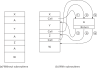
\includegraphics[trim = 30mm 10mm 0mm 0mm,clip,scale=0.9]{imgBook/routines_C8F2_PyP.pdf} \end{textblock}
    \begin{textblock}{100}(10,12)
    Las instruciones para llamar y retornar de una\\ subrutina utilizan un lugar donde \textbf{almacenar\\ la dirección previa del PC}.\\
    \bigskip
    \uncover<2->{
    Este lugar puede ser la pila (\emph{stack})\\ o puede ser un registro específico.\\
    }
    \bigskip
    \uncover<3->{
    \textcolor{verdeuca}{La implementación, puede ser soportada por\\
    completo por una instrucción o requerir de más\\ instrucciones.}\\
    }
    \bigskip
    \uncover<4->{
    En LC-3, el \emph{call} es implementado de forma similar a un JMP,\\ con la diferencia que deja en un registro específico el PC anterior.\\
    \vspace{0.2cm}
    El \emph{return} es implementado por la instruccción JMP,\\ usando un registro específico como fuente.\\
    }
    \end{textblock}
\end{frame}

\begin{frame}[t,fragile]
    \frametitle{Instrucciones de \emph{Call} y \emph{Return}}
    \begin{textblock}{65}(83,10)
    \small Formato instrucción \emph{Call}\\ \vspace{0.2cm}
    \includegraphics[scale=0.7]{imgBook/lc3_instruction_call_PyP-layer1.pdf} \end{textblock}
    \begin{textblock}{65}(83,30)
    \small Ejemplo Instrucción JSR\\ \vspace{0.2cm}
    \includegraphics[scale=0.7]{imgBook/lc3_instruction_call_PyP-layer2.pdf} \end{textblock}
    \begin{textblock}{65}(83,50)
    \small Ejemplo Instrucción JSRR\\ \vspace{0.2cm}
    \includegraphics[scale=0.7]{imgBook/lc3_instruction_call_PyP-layer3.pdf} \end{textblock}
    \begin{textblock}{65}(83,70)
    \small Instrucción RET\\ \vspace{0.2cm}
    \includegraphics[scale=0.662]{imgBook/lc3_jump_instruction_PyP-layer2.pdf} \end{textblock}
    \begin{textblock}{65}(10,12)
    En LC-3 se proveen dos formatos para llamar a subrutinas.\\
    \uncover<2->{
    \begin{itemize}
     \item \textbf{JSR}: Direccionamiento relativo al PC.
     \item \textbf{JSRR}: Direccionamiento por registro.
    \end{itemize}
    }
    \uncover<3->{
    \textcolor{verdeuca}{
    En ambos formatos, una vez calculada la dirección destino, el valor previo de PC
    o \textbf{dirección de retorno se almacena en el registro \texttt{R7}}.}\\
    }
    \bigskip
    \uncover<4->{
    La instrucción \textbf{RET} es la misma instrucción que JMP.
    Se codifica seteando de forma fija el registro \texttt{R7} como destino del salto.\\
    \vspace{0.2cm}
    \textcolor{verdeuca}{Registro donde queda la dirección de retorno.}
    }
    \end{textblock}
\end{frame}

\begin{frame}[t,fragile]
    \frametitle{Pila (\emph{stack})}
    La forma más común de implementar una pila es en memoria.
    \uncover<2->{
    \textcolor{verdeuca}{El \emph{stack} corresponde a una secuencia de posiciones de memoria sobre las que se lleva registro de la primer posición.}\\
    }
    \vspace{0.2cm}
    \uncover<3->{
    Se utilizan dos mecanismos, uno para \textbf{cargar datos} (\emph{push}) y otro para \textbf{retirar datos} (\emph{pop})
    \begin{center}
    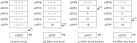
\includegraphics[scale=0.8]{imgBook/stack_in_memory_C8F9_PyP.pdf}
    \end{center}
    }
    \uncover<4->{
    En LC-3, por convención se utiliza el registro R6 como puntero al tope de la pila.\\
    \textcolor{verdeuca}{Este apunta a la primera posición ocupada de la pila.}
    }
\end{frame}

\begin{frame}[t,fragile]
    \frametitle{Mecanismo de \emph{Push} y \emph{Pop}}
    \begin{textblock}{65}(10,12)
    \uncover<1->{
    Para realizar un \textbf{PUSH} se deben ejecutar las siguientes instrucciones:\\
    }
    \uncover<2->{
    \vspace{0.3cm}
    \hspace{2cm} \texttt{ADD R6, R6, \#-1}\\
    \hspace{2cm} \texttt{STR Rx, R6, \#0}\\
    \vspace{0.3cm}
    Las dos instruccciones realizan:
    }
    \begin{enumerate}
     \item<2-> Decrementa el puntero al tope de la pila, apuntando a la nueva posición de memoria que debe ser escrita.
     \item<3-> Escribe en memoria el registro \texttt{Rx}, en la posición de memoria apuntada por el tope de la pila.
    \end{enumerate}
    \end{textblock}
    \begin{textblock}{65}(85,12)
    \uncover<4->{
    Para realizar un \textbf{POP} se deben ejecutar las siguientes instrucciones:\\
    }
    \uncover<5->{
    \vspace{0.3cm}
    \hspace{2cm} \texttt{LDR Rx, R6, \#0}\\
    \hspace{2cm} \texttt{ADD R6, R6, \#1}\\
    \vspace{0.3cm}
    Las dos instruccciones realizan:
    }
    \begin{enumerate}
     \item<5-> Lee de memoria el dato apuntado por el tope de la pila y lo escribe en el registro \texttt{Rx}.
     \item<6-> Incrementa el puntero al tope de la pila, apuntando a la última posición de memoria ocupada en la pila.
    \end{enumerate}
    \end{textblock}
\end{frame}

\begin{frame}[t,fragile]
    \frametitle{Organización de la memoria}
    \begin{textblock}{65}(96,10) 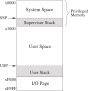
\includegraphics[scale=0.7]{imgBook/lc3_memory_regions.pdf} \end{textblock}
    \begin{textblock}{80}(10,12)
    En LC-3 tiene un espacio de direccionamiento\\ de 16 bits (\texttt{0x0000} a \texttt{0xFFFF}).\\
    \bigskip
    \uncover<2->{
    Este espacio está dividido de la siguiente forma:
    }
    \begin{itemize}
     \item<2-> \textcolor{naranjauca}{\texttt{0x0000} a \texttt{0x2FFF}} - \emph{System space}\\
     Memoria privilegiada. Espacio para las estructuras y código del sistema operativo.
     \item<3-> \textcolor{naranjauca}{\texttt{0x3000} a \texttt{0xFDFF}} - \emph{User space}\\
     Memoria sin privilegios. Espacio para todos los programas de usuario.
     \item<4-> \textcolor{naranjauca}{\texttt{0xFE00} a \texttt{0xFFFF}} - \emph{I/O space}\\
     Memoria privilegiada. Espacio donde se mapean los registros de entrada salida.
    \end{itemize}
    \end{textblock}
    \begin{textblock}{140}(10,80)
    \uncover<4->{
    \textcolor{verdeuca}{Notar que existen dos espacios de pila independientes, para supervisor y usuario.}
    }
    \end{textblock}
\end{frame}

\begin{frame}[t,fragile]
    \frametitle{Entrada/Salida - Dispositivo de entrada (\emph{Keyboard})}
    \begin{textblock}{65}(100,25) \includegraphics[scale=1]{imgBook/lc3_device_registers-layer1.pdf} \end{textblock}
    \begin{textblock}{75}(10,12)
    Para administrar los caracteres que llegan desde el teclado se utilizan \textbf{dos registros}.\\
    \bigskip
    \begin{itemize}
     \item<2-> \textcolor{naranjauca}{\texttt{0xFE02}} - \textbf{\texttt{KBDR}} (\emph{Keyboard Data Register})\\
     Mantiene en los 8 bits menos significativos el caracter que fue presionado.
     \item<3-> \textcolor{naranjauca}{\texttt{0xFE00}} - \textbf{\texttt{KBSR}} (\emph{Keyboard Status Register})\\
     Utiliza solo el bit más significativo como señal de sincronización.
    \end{itemize}
    \end{textblock}
    \begin{textblock}{140}(10,60)
    \uncover<4->{
    \textcolor{verdeuca}{
    Si \texttt{KBSR[15]} = 1, el código ASCII en \texttt{KBDR[7:0]} es válido y aún no fue leído.\\
    En este estado el teclado no puede enviar una nueva tecla.\\}
    }
    \bigskip
    \uncover<5->{
    \textcolor{verdeuca}{
    Si \texttt{KBSR[15]} = 0, el código ASCII en \texttt{KBDR[7:0]} es invalido.\\
    En este estado el teclado puede escribir la nueva tecla y cambiar el estado.\\}
    }
    \end{textblock}
\end{frame}

\begin{frame}[t,fragile]
    \frametitle{Entrada/Salida - Entrada mapeada a memoria}
    \begin{textblock}{65}(2,12) \includegraphics[scale=0.7]{imgBook/lc3_memory_mapped_datapath-layer1.pdf} \end{textblock}
    \begin{textblock}{50}(100,20)
    En este caso, cuando se carga el registro \texttt{MAR} \textcolor{verdeuca}{se identifica si la dirección es de un registro de entrada/salida.}\\
    \bigskip
    \uncover<2->{
    En vez de leer de memoria, la lógica de control se encarga de \textbf{seleccionar el registro que se busca leer}, \textcolor{verdeuca}{guardando su valor en el registro \texttt{MDR}.}
    }
    \end{textblock}
\end{frame}

\begin{frame}[t,fragile]
    \frametitle{Entrada/Salida - Dispositivo de salida (\emph{Monitor})}
    \begin{textblock}{65}(100,25) \includegraphics[scale=1]{imgBook/lc3_device_registers-layer2.pdf} \end{textblock}
    \begin{textblock}{75}(10,12)
    Para administrar los caracteres a imprimir en pantalla se utilizan \textbf{dos registros}.\\
    \bigskip
    \begin{itemize}
     \item<2-> \textcolor{naranjauca}{\texttt{0xFE06}} - \textbf{\texttt{DDR}} (\emph{Display Data Register})\\
     Mantiene en los 8 bits menos significativos el caracter que quiere ser escrito en pantalla.
     \item<3-> \textcolor{naranjauca}{\texttt{0xFE04}} - \textbf{\texttt{DSR}} (\emph{Display Status Register})\\
     Utiliza solo el bit más significativo como señal de sincronización.
    \end{itemize}
    \end{textblock}
    \begin{textblock}{140}(10,60)
    \uncover<4->{
    \textcolor{verdeuca}{
    Si \texttt{DSR[15]} = 1, el código ASCII en \texttt{DDR[7:0]} fue leído por el monitor.\\
    Ahora se puede escribir un nuevo caracter y setear a cero la señal de sincronización.\\}
    }
    \bigskip
    \uncover<5->{
    \textcolor{verdeuca}{
    Si \texttt{DSR[15]} = 0, el código ASCII en \texttt{DDR[7:0]} está a la espera de ser leído por el monitor.\\
    En este estado, se debe esperar a que el monitor lea para escribir el nuevo caracter.\\}
    }
    \end{textblock}
\end{frame}

\begin{frame}[t,fragile]
    \frametitle{Entrada/Salida - Salida mapeada a memoria}
    \begin{textblock}{65}(2,12) \includegraphics[scale=0.7]{imgBook/lc3_memory_mapped_datapath-layer2.pdf} \end{textblock}
    \begin{textblock}{50}(100,20)
    En este caso, cuando se carga el registro \texttt{MAR} \textcolor{verdeuca}{se identifica si la dirección es de un registro de entrada/salida.}\\
    \bigskip
    \uncover<2->{
    En vez de escribir en memoria, la lógica de control se encarga de \textbf{activar la señal para escribir el registro}, \textcolor{verdeuca}{tomando el valor del registro \texttt{MDR}.}
    }
    \end{textblock}
\end{frame}

\begin{frame}[t,fragile]
    \frametitle{Entrada/Salida - Mapeada a memoria}
    \begin{textblock}{65}(2,12) \includegraphics[scale=0.7]{imgBook/lc3_memory_mapped_datapath-layer3.pdf} \end{textblock}
    \begin{textblock}{45}(105,13)
    Los mecanismos de mapeo a memoria son similiares para \textcolor{verdeuca}{lectura y escritura}.\\
    \bigskip
    \uncover<2->{
    Mapear a memoria implica lógica que decide \textcolor{verdeuca}{que direcciones corresponden a que almacenamiento.}
    }
    \end{textblock}
    \begin{textblock}{140}(10,60)
    \uncover<3->{
    Este mecanismo se complementa con \textbf{interrupciones}, que permite despertar rutinas para resolver una acción de entrada/salida específica.\\
    }
    \bigskip
    \uncover<4->{
    \textcolor{gray}{La solución para administrar un espacio de entrada/salida independiente,\\ es similiar a tener otra memoria accedida por instrucciones diferentes.}
    }
    \end{textblock}
\end{frame}

\begin{frame}[t,fragile]
    \frametitle{Resumen}
    Definir un ISA implica minimamete,\\
    \vspace{0.4cm}
    \begin{itemize}
    \setlength\itemsep{0.4cm}
    \item<2-> Definir la \textbf{interfaz} entre el software y el hardware del procesador.
    \item<3-> Definir sus \textbf{instrucciones}, su comportamiento y codificación.
    \item<4-> Definir los tamaños y propiedades de la \textbf{memoria}.
    \item<5-> Definir como se organizará la memoria y administrará la \textbf{pila}.
    \item<6-> Definir los modos de \textbf{direccionamiento} y su alcance dependiendo de cada instrucción.
    \item<7-> Definir los mecanismos de \textbf{protección} con los que contará el procesador.
    \item<8-> Definir el soporte para \textbf{entrada/salida}, administración de dispoositivos e \textbf{interrupciones}.
    \end{itemize}
\end{frame}

\begin{frame}[fragile]
    \frametitle{Bibliografía}
    \begin{itemize}
    \setlength\itemsep{0.0cm}
%       \item[-] \small David Money Harris, Sarah L. Harris\\
%       \textbf{``Digital Design and Computer Architecture''} Second Edition, Morgan Kaufmann\\
%       \item[-] \small John L. Hennessy, David A. Patterson\\
%       \textbf{``Computer Architecture: A Quantitative Approach''} Sixth Edition, Morgan Kaufmann\\
    \item[-] \small Yale N. Patt, Sanjay J. Patel\\
    \textbf{``Introduction to Computing Systems''} - Third Edition - McGraw-Hill\\
    \begin{itemize}
    \item Chapter 4 - The von Neumann Model $\rightarrow$ Pag. 121-137
    \item Chapter 5 - The LC-3 $\rightarrow$ Pag. 145-177
    \item Chapter 8 - Data Structures $\rightarrow$ Pag. 263-268
    \item Chapter 9 - I/O $\rightarrow$ Pag. 313-327
    \end{itemize}
%       \item[-] \small M. Morris Mano\\
%       \textbf{``Diseño Digital''} - Tercera Edicion, Pearson\\  
    \end{itemize}
\end{frame}

\begin{frame}[plain]
    \begin{center}
    \vspace{2cm}
    \huge ¡Gracias!\\
    \vspace{2cm}
    \end{center}
\end{frame}

\end{document}

